\documentclass[a4paper,12pt]{article} % тип документа

% Поля страниц
\usepackage[left=2.5cm,right=2.5cm,top=1.5cm,bottom=2cm,bindingoffset=0cm]{geometry}
    
% Отступ после заголовка
\usepackage{indentfirst}

% Картинки
\usepackage{graphicx}
\graphicspath{{images/}}
\usepackage{placeins}

% Таблицы
\usepackage{booktabs}
% \usepackage{floatrow}
\usepackage{subcaption}

% Русский язык
\usepackage{cmap}  % поиск в PDF
\usepackage{mathtext}  % русские буквы в формулах
\usepackage[T2A]{fontenc}  % кодировка
\usepackage[utf8]{inputenc}  % кодировка исходного текста
\usepackage[english,russian]{babel}  % локализация и переносы

% Математика
\usepackage{amsmath}

% Ссылки TODO
% \usepackage[unicode=true]{hyperref}
% \usepackage[T1]{fontenc}

\begin{document}

\begin{center}   
	\large{\textbf{Работа 2.2.5 \\ Определение теплоты испарения жидкости}}\\
\end{center}

\section{Аннотация}

\noindent\textbf{Цель работы:}
1) определение вязкости воды по измерению объёма жидкости, протекшей через капилляр; 2) определение вязкости других жидкостей путём сравнения скорости их перетекания со скоростью перетекания воды.
	
\smallskip
\noindent\textbf{В работе используются:}
сосуд Мариотта; капиллярная трубка; мен-зурка; секундомер; стакан; микроскоп на стойке.

\section{Теоретические сведения}

\subsection*{Абсолютный метод}

Формула Пуазейля для расхода жидкости через сечение трубки:

\begin{equation}
	Q = \pi \frac{P_1-P_2}{8 \eta l} R^4
\end{equation}

Число Рейнольдса:
\begin{equation}
	Re = \frac{v R \rho}{\eta} = \frac{2\frac{\rho v^2}{2}}{\eta \frac{v}{R}}
\end{equation}

Согласно уравнению Бернулли:
\begin{equation}
	\frac{\rho v^2}{2} = P_0 - P
\end{equation}

В гладких трубах круглого сечения переход от ламинарного движения к турбулентному происходит при $Re \approx 1000$.

Ламинарное движение жидкости при переходе ее из широкого сосуда в капилляр устанавливается не сразу, а после того, как она пройдет расстояние:
\begin{equation}
	a \approx 0.2R \cdot Re
\end{equation}

\subsection*{Относительный метод}

Заменяя в формуле Пуазейля $Q_v$ на $-dV/dt$ и $P_1 - P_2$ на $\rho g h$, получим
\begin{equation}
	\frac{\rho_1}{\eta_1}t_1 = \frac{\rho_2}{\eta_2}t_2 = \frac{\rho_3}{\eta_3}t_3 = ...
\end{equation}

Проведя опыты с водой, а затем с исследуемой жидкостью, найдем
\begin{equation}
	\eta_x = \eta_0\frac{\rho_x}{\rho_0}\frac{t_x}{t_0}
\end{equation}

\section{Используемое оборудование}

\subsection*{Абсолютный метод}

Установка для измерения вязкости воды изображена на (рис. \ref{setup1}).
Вода заполняет сосуд Мариотта и вытекает через калиброванную капиллярную трубку, укрепленную в нижней части его боковой стенки. Сосуд Мариотта позволяет поддерживать постоянным перепад давления $P_1 - P_2$ на концах капилляра, несмотря на то, что уровень жидкости при ее вытекании понижается. Это достигается с помощью трубки В, открытой в атмосферу и проходящей через пробку, герметично закрывающую сосуд. \par
Величина перепада давления $P_1 - P_2$ определяется высотой столба воды $h$ между осью капиллярной трубки А и нижним концом вертикальной трубки В. Высота столба измеряется с помощью микроскопа М, укрепленного на вертикально перемещающемся плунжере. Смещение плунжера определяется по миллиметровой шкале, снабженной нониусом. Объем вытекшей жидкости измеряется мензуркой П. Время истечения определяется по секундомеру. Длина капиллярной трубки измеряется миллиметровой линейкой, диаметр ---
микроскопом МИР.

\begin{figure}[h!]
    \centering
    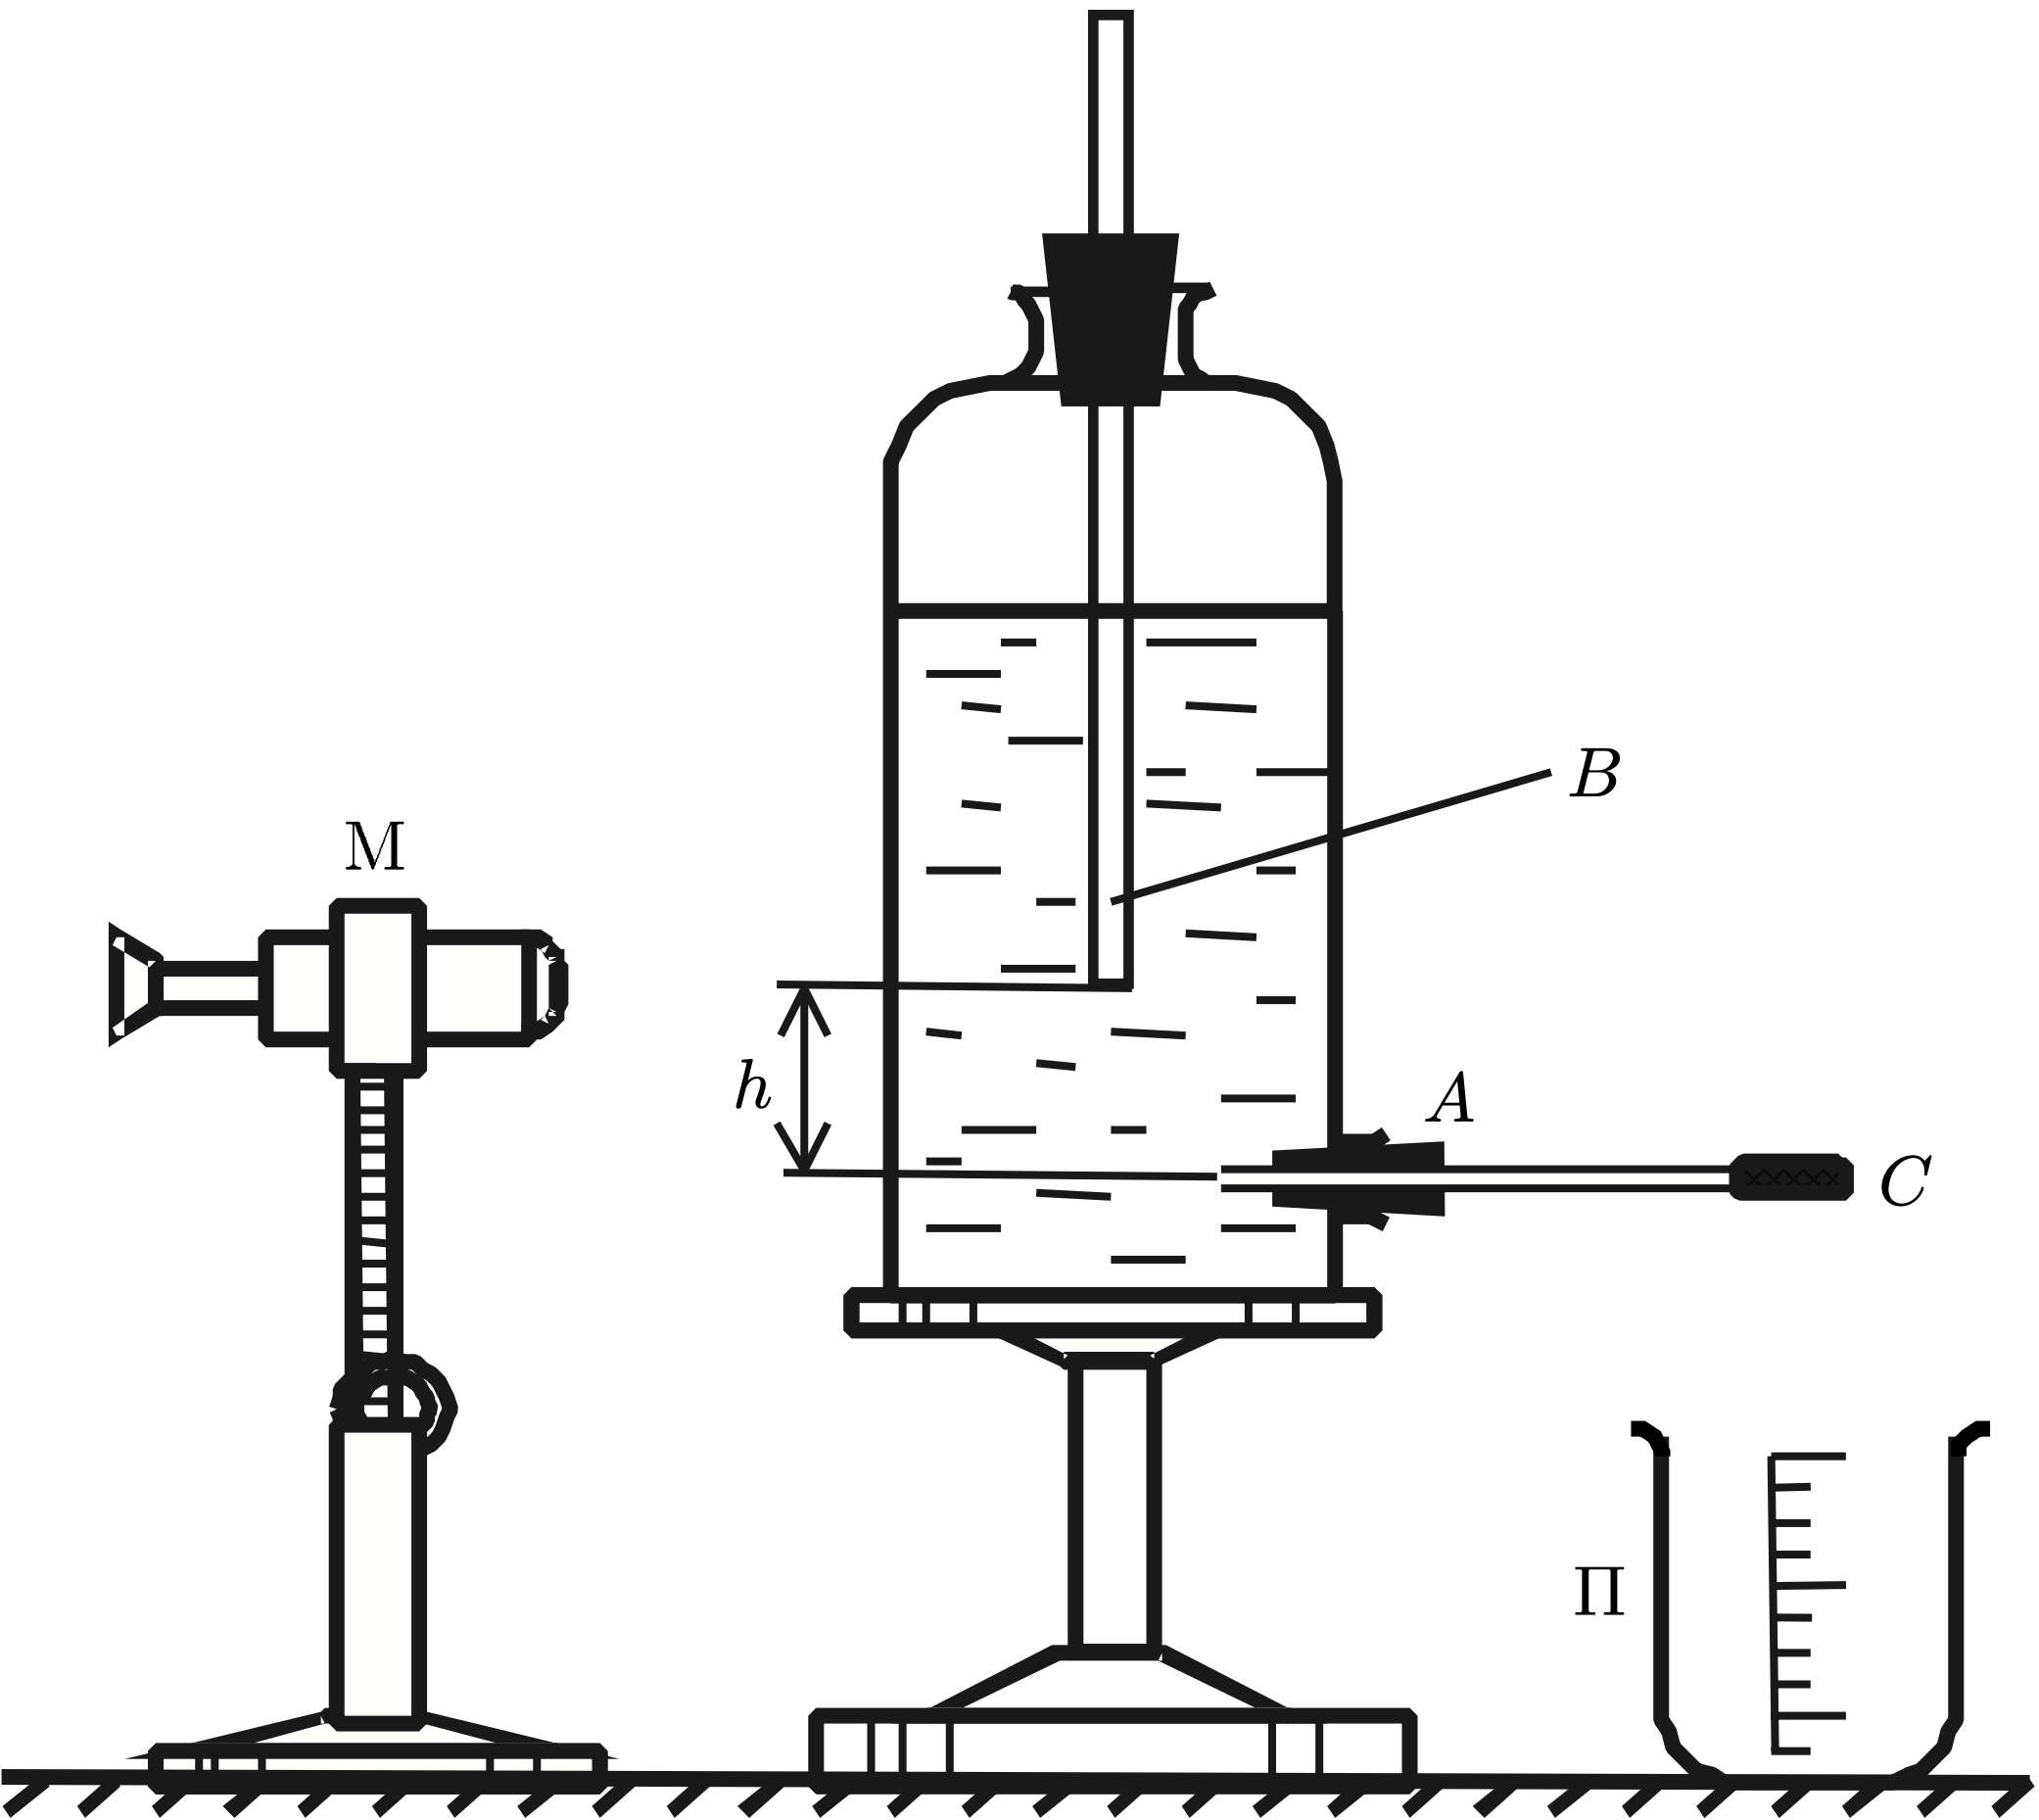
\includegraphics[width=0.44\textwidth]{установка1}
    \caption{Схема установки для определения вязкости воды}
	\label{setup1}
\end{figure}

\FloatBarrier

\subsection*{Относительный метод}

\begin{figure}[h!]
    \centering
    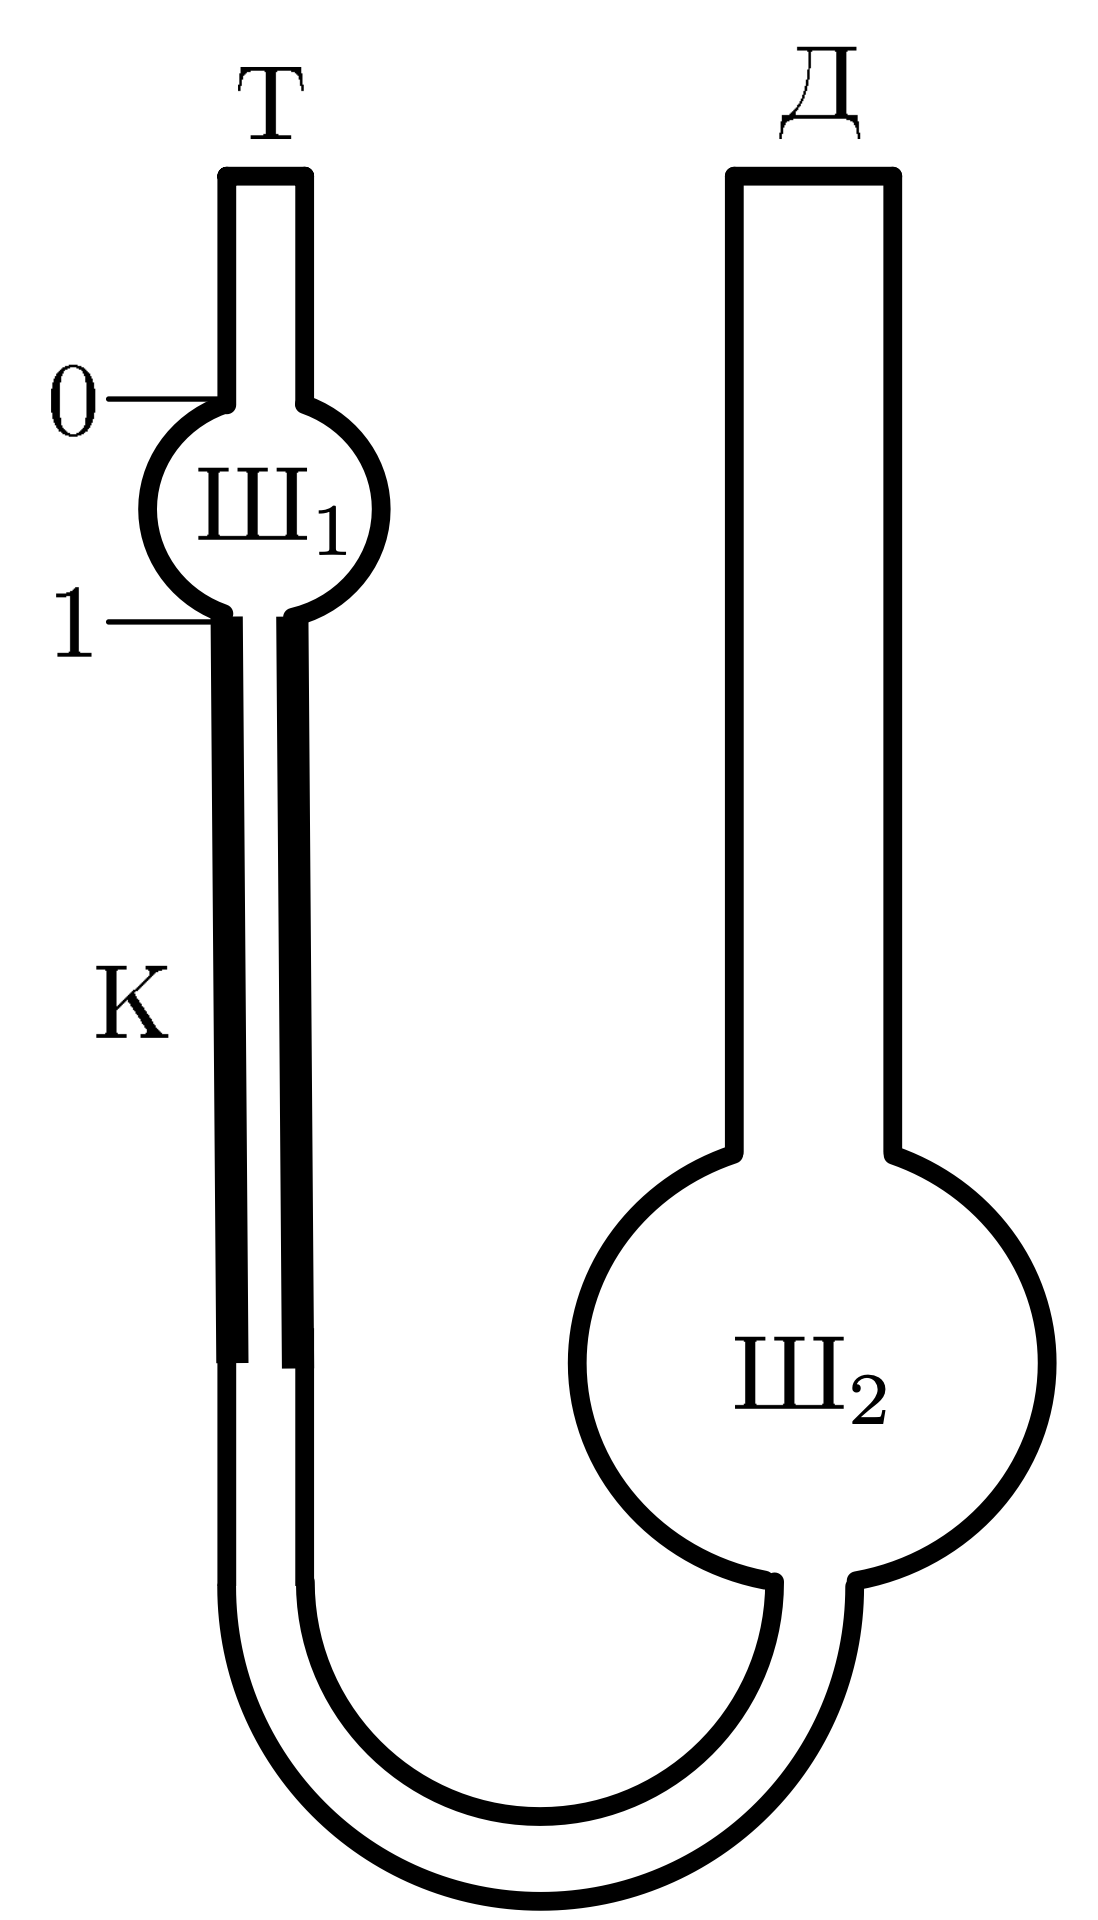
\includegraphics[height=0.32\textwidth]{установка2}
    \caption{Схема установки для определения вязкости воды}
	\label{setup2}
\end{figure}

Вискозиметр Оствальда (рис. \ref{setup2}) представляет собой U-образную стеклянную трубку.

В широкую трубку вискозиметра вливают определенное количество воды, вязкость \( \eta \) которой известна. С помощью резиновой груши, подсоединенной к узкой трубке \(Т\), засасывают воду так, чтобы её мениск поднялся немного выше метки «0». Сняв грушу с трубки и удерживая вискозиметр в вертикальном положении, дают возможность воде свободно протекать через капилляр \(К\). Когда мениск проходит метку «0», включают секундомер, и выключают его, когда мениск проходит метку «1». Таким образом измеряют время \( t_0 \), за которое объем воды \( V \), заключенный между метками в шарике \(Ш_1\), протекает через капилляр.


\FloatBarrier

% \section{Методика измерений}

% \section{Результаты измерений и обработка данных}

% \section{Обсуждение результатов}

\end{document}
